\chapter{Question 1}
\label{question-1}
\section{Question}

\begin{itemize}
\item For the text you saved for the 10000 URIs from A1, Q2:
	\begin{itemize}
	\item Use the “boilerpipe” software to remove the HTML templates from all HTML pages (document how many pages link from the tweets were non-HTML and had to be skipped).
	\item \url{https://code.google.com/p/boilerpipe/}
	\item WSDM 2010 paper: \url{http://www.l3s.de/~kohlschuetter/boilerplate/}
	\end{itemize}
\item For how many of the 10000 URIs was boilerpipe successful?
	\begin{itemize}
	\item Compare the total words, unique words, and byte sizes before and after use of boilerpipe.
	\end{itemize}
\item For what classes of pages was it successful?
\item For what classes of pages was it unsuccessful?
\item Provide examples of both successful and unsuccessful removals and discuss at length.
\end{itemize}


\section{Solution}
\begin{itemize}
\item For this assignment I used the boilerpipe library on python.
\item I installed the library on the linux machine using the command `sudo pip install boilerpipe'.
\item I saved the HTML files that I downloaded from the first assignment to my folder located at \url{www.cs.odu.edu/~kahmed/cs751/a3/} so I could use them as URIs to be used for the boilerpipe script.
\item From the 10000 URIs I was able to download the HTML files for 9978 URIs. The files were not created for the URIs which returned a 404 response. From the remaining URIs I was able to retrieve 8476 URIs as some of them did not have any HTML data.
\item From the 8476 URIs that remained after successful retrieval of HTML content, the boilerpipe was successful for 6275 URIs. Below is a comparison of the data before and after running them through the boilerpipe script. \\*
	\begin{minipage}{\linewidth}
		\centering
			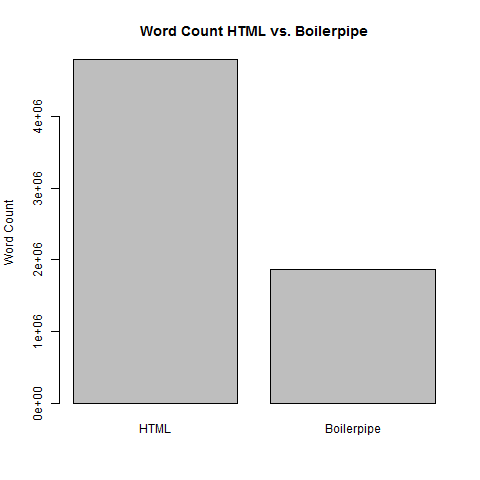
\includegraphics[scale=0.55]{figures/wordCount.png}
		\captionof{figure}{Word Count for HTML vs. Boilerpipe}
		\label{wordCount}
	\end{minipage}
	\begin{minipage}{\linewidth}
		\centering
			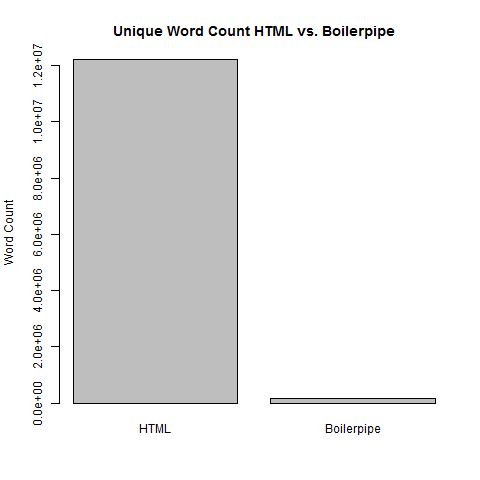
\includegraphics[scale=0.55]{figures/uniqueWord.png}
		\captionof{figure}{Unique Word Count for HTML vs. Boilerpipe}
		\label{uniqueWord}
	\end{minipage}
	\begin{minipage}{\linewidth}
		\centering
			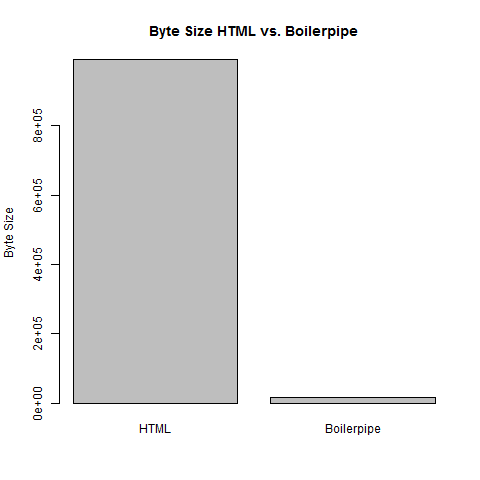
\includegraphics[scale=0.55]{figures/byteSize.png}
		\captionof{figure}{Byte Size for HTML vs. Boilerpipe}
		\label{byteSize}
	\end{minipage}
\item I used python scripts to retrieve this information for individual files and then used Microsoft Excel to get the total number of words in each case.
\end{itemize}

\subsection{Boilerpipe Successful}
\begin{itemize}
\item I selected a few URIs for which the boilerpipe was successful.
\item A few examples of successful boilerpipe retrieval are:
	\begin{itemize}
	\item \url{http://her-life-and-health.com/?a=adm}
	\item \url{https://play.google.com/store/apps/details?id=com.maoline.kindan.droid}
	\end{itemize}
\item I noticed that the successful ones had HTML elements such as `<div>', `<p>', etc. with text enclosed within them.
\end{itemize}

\subsection{Boilerpipe Unsuccessful}
\begin{itemize}
\item I performed the same activity of selecting URIs for which boilerpipe was unsuccessful.
\item A few examples of unsuccessful boilerpipe retrieval are:
	\begin{itemize}
	\item \url{http://jsm084.wix.com/joy1063}
	\item \url{http://instagram.com/p/ysl6lgFD_H/}
	\end{itemize}
\item Upon further investigation of these HTML pages, I came to a conclusion that the HTML pages for these URIs had only HTML script tags such as `<script>' within them.
\item The boilerpipe is designed the ignore the data enclosed within these script tags.
\item It is designed to check for data enclosed within the block elements like `<div>', '<p>', etc.
\item For the example listed above, the Instagram URI ran external scripts for fetching the data to be displayed. The HTML page basically consists of scripts to be called and the necessary arguments to be passed to the script to display the necessary content which in this case was a picture and the comments for that picture from other Instagram users.
\item This is applicable for the rest of the URIs for which boilerpipe was unsuccessful.
\end{itemize}

\newpage
\section{Code Listing}

\lstinputlisting[language=Python,breaklines = true,frame=single,caption={Python program for retrieving the boilerpipe data.},label=lst:q1-1,captionpos=b,numbers=left,showspaces=false,showstringspaces=false,basicstyle=\footnotesize]{pythonFiles/boilerPipe.py}
\newpage
\lstinputlisting[language=Python,breaklines = true,frame=single,caption={Python program for retrieving the unique word count from HTML.},label=lst:q1-1,captionpos=b,numbers=left,showspaces=false,showstringspaces=false,basicstyle=\footnotesize]{pythonFiles/readHtml.py}
\newpage
\lstinputlisting[language=Python,breaklines = true,frame=single,caption={Python program for retrieving the word count for individual file.},label=lst:q1-1,captionpos=b,numbers=left,showspaces=false,showstringspaces=false,basicstyle=\footnotesize]{pythonFiles/wordCount.py}
\newpage
\lstinputlisting[language=Python,breaklines = true,frame=single,caption={Python program for retrieving unique word list for boilerpipe successful files.},label=lst:q1-1,captionpos=b,numbers=left,showspaces=false,showstringspaces=false,basicstyle=\footnotesize]{pythonFiles/wordList.py}

\newpage
\lstinputlisting[language=R,breaklines = true,frame=single,caption={R program for generating the bar plot for total word count for HTML vs. Boilerpipe}, label=lst:q1R1,captionpos=b,numbers=left,showspaces=false,showstringspaces=false,basicstyle=\footnotesize]{rFiles/wordCount.R}
\lstinputlisting[language=R,breaklines = true,frame=single,caption={R program for generating the bar plot for unique word count for HTML vs. Boilerpipe}, label=lst:q1R1,captionpos=b,numbers=left,showspaces=false,showstringspaces=false,basicstyle=\footnotesize]{rFiles/uniqueWord.R}
\lstinputlisting[language=R,breaklines = true,frame=single,caption={R program for generating the bar plot for byte size of HTML vs. Boilerpipe}, label=lst:q1R1,captionpos=b,numbers=left,showspaces=false,showstringspaces=false,basicstyle=\footnotesize]{rFiles/byteSize.R}